\documentclass[conference]{IEEEtran}


\let\chapter\section
\let\section\subsection
\let\subsection\subsubsection
\let\subsubsection\paragraph

\usepackage[bahasa]{babel}
\usepackage{cite}
\usepackage{graphicx}
\usepackage{listings}
\usepackage{url}
\usepackage{tabto}
\begin{document}
	\title{Metode Pengaliran Data Audio melalui Sistem Penyeimbang Muat berbasis HAProxy}
\author{\IEEEauthorblockN{Bahrul Halimi\IEEEauthorrefmark{1},
        Putu Wiramaswara Widya\IEEEauthorrefmark{2}}
    \IEEEauthorblockA{Fakultas Teknologi Informasi,
        Institut Teknologi Sepuluh Nopember\\
        Surabaya\\
        Email: \IEEEauthorrefmark{1}bahrul.halimi11@mhs.if.its.ac.id,
			\IEEEauthorrefmark{2}wiramaswara11@mhs.if.its.ac.id}}
	
\maketitle
\begin{abstract}
    We propose ...
\end{abstract}
\begin{IEEEkeywords}
    \textit{Streaming}, HAProxy, Icecast, Penyeimbang Muat, Internet Radio.
\end{IEEEkeywords}


	
\chapter{Pendahuluan}

\section{Latar Belakang}

Informasi menyebar dari lokasi ke lokasi lain dengan berbagai macam bentuk media, mulai dari media udara melalui percakapan sehari-hari secara langsung hingga media Internet yang bisa dijangkau oleh dua pihak yang berjauhan. Akhir-akhir ini, media Internet menjadi salah satu sarana yang mulai banyak dan lumrah digunakan untuk proses penyebaran dan penerimaan informasi.

Salah satu aplikasi penyebaran informasi melalui Internet adalah melalui radio Internet yang dialirkan melalui aliran atau \textit{streaming} berkas suara melalui jaringan Internet berbasis TCP/IP. Proses pengaliran data multimedia sendiri sudah lama dikenal masyarakat Indonesia. Semakin murahnya dan banyaknya penggunaan Internet di seluruh dunia memunculkan banyaknya penyedia layanan radio Internet baik pengguna secara individu maupun perusahaan penyiaran yang sudah besar. Banyak radio lokal yang pada awalnya bersiaran secara analog melalui frekuensi radio FM/AM pada akhirnya membuka peluang dirinya agar bisa bersiaran melalui jaringan Internet sehingga radio mereka dapat diakses secara luas tanpa adanya batasan geografis. 

Berbeda dengan radio analog, proses penyiaran radio Internet dilakukan dalam mekanisme yang tidak sederhana. Suara atau audio siaran tidak disalurkan melalui gelombang radio dalam bentuk analog suara, melainkan dalam bentuk data audio digital dalam berbagai format yang umumnya sudah terkompresi. Data ini kemudian disebarkan melalui jaringan Internet ke pengguna dengan rasio 1:1, yang berarti satu data audio dikirimkan ke setiap satu pendengar yang mengaksesnya. Hal ini menyebabkan radio Internet rentan terhadap masalah ketersediaan (\textit{avialibility}) yang terjadi ketika server penyedia tidak mampu melayani semakin banyaknya pendengar.

Pada kesempatan ini, dilakukan penelitian mengenai penggunaan sistem penyeimbang muat pada server radio Internet untuk memaksimalkan ketersediaan server pada beban puncak. Sistem pembagi muat akan membantu mengatur muatan permintaan data suara dari pengakses radio Internet ke banyak komputer server yang menyediakan isi konten siaran yang sama. Untuk perangkat lunak implementasi, penelitian ini menggunakan server berbasis Icecast (\url{http://icecast.org}) yang memiliki lisensi terbuka dan protokol yang kompatibel dengan HTTP dengan sistem pembagi muat berbasis HAProxy (\url{http://haproxy.org}).

\section{Permasalahan}
Berikut beberapa hal yang menjadi rumusan masalah dalam pengerjaan penelitian ini :
\begin{enumerate}
    \item Bagaimana menyeimbangkan muatan kerja server yang menyiarkan audio ke pendengar ketika ada banyak permintaan secara bersamaan?
    \item Bagaimana menyediakan banyak server untuk melayani permintaan pendengar dengan satu sumber aliran dari pengirim?

\end{enumerate}

\section{Batasan Masalah}
Dari permasalahan yang diuraikan di atas, terdapat beberapa batasan masalah pada penelitian ini, yaitu :
\begin{enumerate}
    \item Aliran data multimedia yang didukung hanya audio.
\end{enumerate}

\section{Tujuan dan Manfaat}
Penelitian ini dibuat dengan beberapa tujuan sebagai berikut :
\begin{enumerate}
\item Mencari tahu manfaat penggunaan sistem penyeimbangan muat pada sistem pengaliran data multimedia berbasis audio.
\end{enumerate}


\chapter{Tinjauan Pustaka}
\section{Teori Penunjang}
\begin{enumerate}
    \item HAProxy
    
    HAProxy ( High Availability Proxy ) merupakan salah satu sistem penyeimbang muat handal pada protokol TCP/HTTP. Sistem yang digunakannya akan membagi beban kerja ke sekumpulan server untuk memaksimalkan kerjanya.
    
    Beberapa alasan mengapa HAProxy ini banyak digunakan adalah :
    \begin{enumerate}
        \item Sangat cepat.
        \item Efisien, dengan 700 permintaan dalam satu detik CPU yang digunakan kurang dari 5\% dan 40MB RAM.
        \item Memungkinkan untuk dilakukan perubahan konfigurasi selama koneksi masih terjadi dan tidak akan mengganggu koneksi tersebut.
        \item Memungkinkan adanya \textit{queue} dalam pengaplikasiannya jika memang koneksi yang masuk terlalu banyak.
    \end{enumerate}
    
    
    \item Icecast
    
    Merupakan kumpulan dari program dan pustaka yang digunakan untuk melakukan \textit{audio streaming} melalui internet. Ada tiga komponen utama di dalamnya yaitu :
    
    \begin{enumerate}
        \item Icecast
        
        Program ini akan menyampaikan data stream audio ke pendengar.
        
        \item Libshout
        
        Adalah sebuah pustaka yang digunakan untuk mengirimkan data ke server. Data ini berasal dari orang yang ingin menyebarkan audionya sehingga bisa didengarkan orang lain.
        
        \item IceS
        
        Program yang akan mengirimkan data audio dari ke server dan disebarkan secara broadcast ke pendengar. Program ini dapat mengirim data audio di dalam media penyimpanan seperti berkas Ogg Vorbis atau suara langsung yang ditangkap sound card.
    \end{enumerate}
    
    \item NodeJS
    
    Merupakan sebuah platform yang dibangun di atas Chrome's JavaScript runtime dengan teknologi V8 yang mendukung proses server yang bersifat \textit{long-running}. Tidak seperti platform modern yang mengandalkan multithreading, NodeJS memilih menggunakan asynchronous I/O eventing. Karena inilah NodeJS mampu bekerja dengan konsumsi memori rendah.
    
    
    
\end{enumerate}

\section{Solusi Sebelumnya}

Beberapa pengembangan terhadap terknologi di atas antara lain:

\begin{enumerate}
    \item GitHub
    
    Sebagai media untuk melakukan \textit{versioning} dalam pengembangan perangkat lunak, pengguna mengharapkan kecepatan akses terhadap halaman pribadinya. Oleh karena itu pengembang Github memanfaatkan fitur \textit{proxy} pada HAProxy untuk membagi kinerja server di dalamnya sehingga pengguna dapat dengan cepat mengakses halaman pribadinya. (mojombo, 2009)
    
    \item Stack Overflow / Server Fault
    
    Pengembangnya jelas menyebutkan bahwa mereka adalah penggemar HAProxy yang telah berhasil me-\textit{load balancing}-kan 2 hingga 3 komputer server yang dimilikinya.
\end{enumerate}

\chapter{Metode Penelitian}

\section{Arsitektur Aplikasi}

Aplikasi akan dibagi menjadi dua bagian yaitu \textbf{Frontend} (yang berhadapan di sisi pendengar atau pengakses) dan \textbf{Backend} (yang berurusan dengan penyiar). 

Pada bagian Frontend, pendengar akan berhadapan dengan server penyeimbang muat berbasis HAProxy yang akan mengarahkan permintaan pendengar ke server yang tersedia untuk melayani. Sementara pada bagian Backend, pengirim atau penyiar akan berhadapan dengan server penerima data aliran audio yang nantinya akan menyebarkan data audio ke seluruh server penyedia.

\begin{figure}
    \centering
    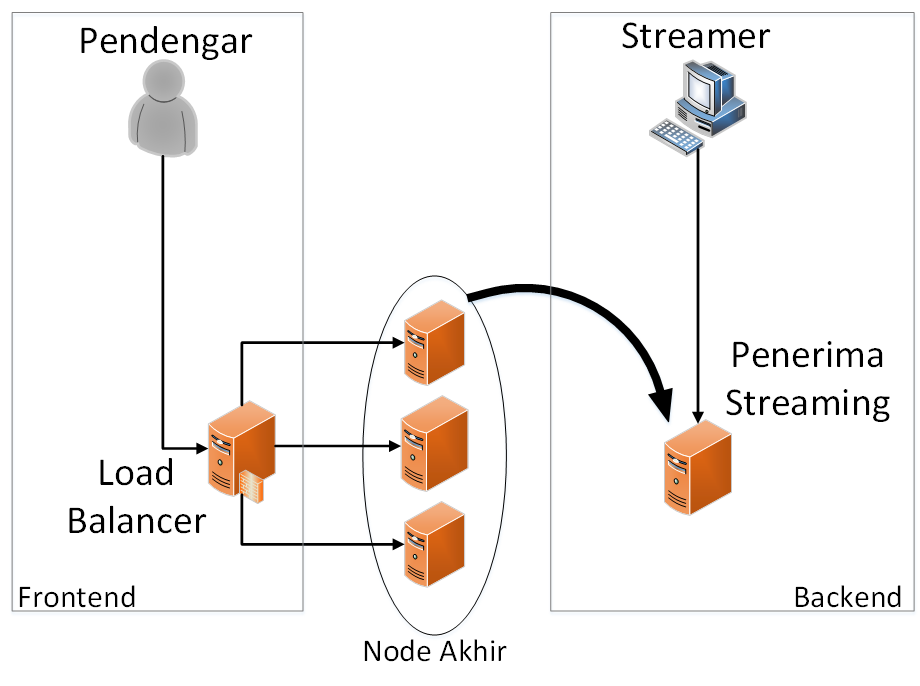
\includegraphics[width=1\linewidth]{arsitektur}
    \caption{Arsitektur Jaringan}
    \label{fig:arsitektur}
\end{figure}

Gambar \ref{fig:arsitektur}  menjelaskan bagaimana interaksi antara server (Frontend dan Backend), pendengar, dan pengirim. Dengan pembagian kerja ini nantinya pendengar hanya akan mengetahui aliran data audio mana saja yang aktif dan pengirim hanya akan mengirim aliran data audio.

\section{Fitur Aplikasi}
\subsection{Pengaliran Data Audio}

Perangkat lunak server IceCast pada awalnya hanya mendukung pengaliran data audio ke satu server saja untuk satu kali proses pengaliran. Fitur Pengaliran Data Audio dalam penelitian ini akan membuat pengaliran data audio tidak hanya tertuju ke satu server, melainkan ke banyak server sekaligus yang dikelola oleh sistem pembagi muat. Sistem akan dibuat setransparan mungkin sehingga pihak penyiar atau pengirim hanya tetap mengakses pengiriman data ke satu alamat server seperti sebelumnya.

Pada Gambar \ref{fig:kirim-server} diagram alir menjelaskan bagaimana pengirim mengirimkan paket audionya ke satu server saja. Pada saat data audio masuk ke server, server akan meneruskan data audio ke node akhir sehingga node akhir memiliki data audio yang sama dengan yang diterima server.

Gambar \ref{fig:kirim-server} menjelaskan apa yang terjadi di bagian backend aplikasi.

\begin{figure}[h]
    \centering
    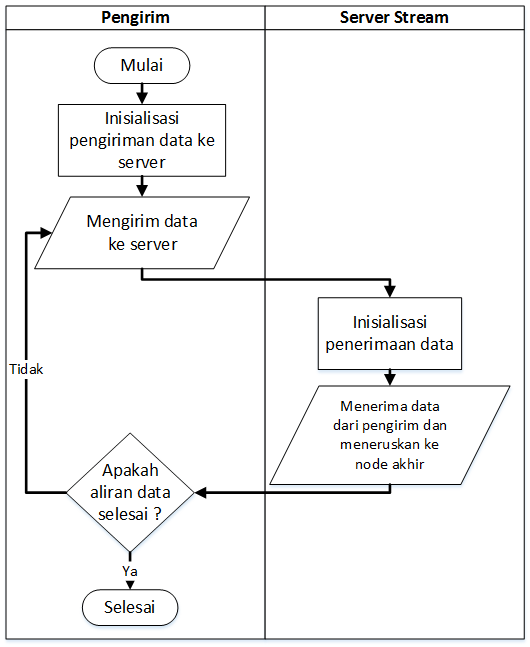
\includegraphics[width=1\linewidth]{kirim-server}
    \caption{Alur Kerja Pengirim dan Server}
    \label{fig:kirim-server}
\end{figure}


\subsection{Penyeimbang Muat}
Penyeimbang muat diakses ketika ada pendengar atau pengakses yang ingin mengakses siaran yang tersedia pada Server. Pada kenyataannya pendengar hanya akan mengakses satu alamat server yang akan memintakan layanan ke Node akhir. Server yang diakses oleh pendengar tidak memiliki layanan yang diminta oleh pendengar, server hanya bertindak sebagai penerus dan penyeimbang muat bagi permintaan yang banyak.

\begin{figure}[h]
    \centering
    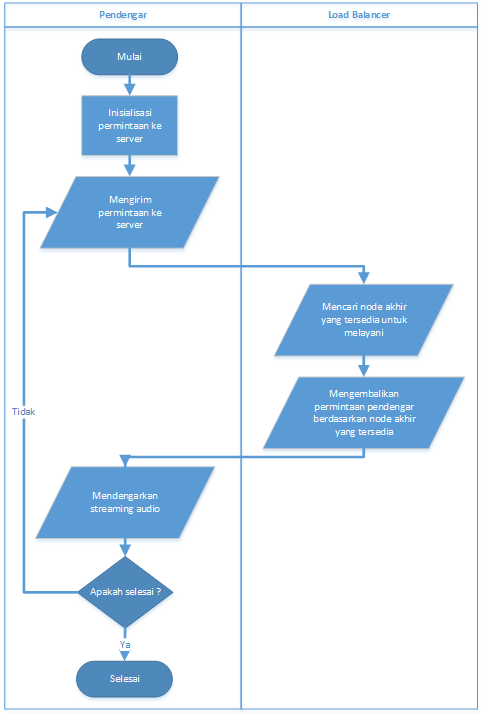
\includegraphics[width=1\linewidth]{dengar-server}
    \caption{Alur Kerja Pendengar dan Server}
    \label{fig:dengar-server}
\end{figure}

Sesuai dengan Gambar \ref{fig:dengar-server}, server yang diakses pengguna adalah server penyeimbang muat yang hanya sebagai jembatan dalam layanan aliran data audio. 

\section{Sarana Yang Digunakan}

Dalam penilitian ini, digunakan beberapa teknologi untuk mengaplikasikan rancangan yang sudah ada, diantaranya:

\begin{enumerate}
    \item Bahasa Pemrograman
    
    Menggunakan nodejs untuk konfigurasi antara pengirim dan server.
    
    \item Editor Teks
    
    Penilitian ini menggunakan editor teks VIM (\url{http://vim.org}) untuk proses implementasi kode.
    
    \item Perangkat Keras
    
    Untuk menunjang fitur penyeimbang muat, digunakan beberapa komputer virtuak di dalam Proxmox. Proxmox menyediakan banyak virtualisasi di dalam satu komputer fisik. Lokasi server Proxmox ada di Laboratorium Arsitektur dan Jaringan Komputer Teknik Informatika ITS.
    
    \item Pengirim data audio
    
    Aplikasi \textit{audio streaming} yang digunakan untuk menguji coba sisi penyiar adalah Mixxx yang memiliki fitur pemutaran musik berbasis Disc Jockey (DJ).
    \end{enumerate}

\chapter{Implementasi}


\section{Sisi Pendengar}
Pada implementasi fitur penyeimbang muat dari sisi pendengar, HAPHAProxy menyediakan satu alamat server yang bisa diakses oleh pendengar dan meneruskannya ke tiga node akhir. Untuk menyokong sistem penyeimbang muat, disediakan tiga Node akhir pada alamat masing-masing \texttt{10.151.36.201}, \texttt{10.151.36.202}, dan \texttt{10.151.36.203}. Ketiga Node akhir ini sudah terpasang server Icecast dengan konfigurasi bawaan. Konfigurasi \texttt{haproxy.cfg} dapat dilihat pada Listing \ref{lst:haproxycfg} berikut.



%\label{lst:haproxycfg}
%\caption{Konfigurasi HAProxy pada penyeimbang muat}
\begin{lstlisting}[breaklines,frame=single]
frontend localnodes
bind *:8000
mode http
default_backend nodes

backend nodes
mode http
balance leastconn
option forwardfor
option httpchk GET /
server ice1 10.151.36.201:8000 check maxconn 100000
server ice2 10.151.36.202:8000 check maxconn 100000
server ice3 10.151.36.203:8000 check maxconn 100000

\end{lstlisting}

Konfigurasi HAProxy di atas berjalan di server dengan alamat 10.151.36.205. Fitur penyeimbang muat ini bekerja pada port 8000 dan akan meneruskan permintaan yang masuk ke tiga node akhir yang sudah dituliskan di dalam konfigurasi. 
\section{Sisi Penyiar/Pengirim}

\subsection{Basis Data}
Dalam penelitian ini digunakan basis data berbasis dokumen MongoDB (\url{http://mongodb.org}) . Secara umum struktur dari basis data dalam penilitian ini terdiri dari tiga koleksi yaitu :

\begin{enumerate}
    \item \textbf{Peers} 
    
    Koleksi ini berisi daftar Node akhir yang bisa digunakan untuk melayani pendengar. Kolom yang digunakan untuk menyimpan informasi node akhir adalah sebagai berikut :
    
    \begin{itemize}
    \item Kolom \texttt{ip} merupakan alamat dari node akhir yang tersedia
    \item Kolom \texttt{online} untuk menginformasikan apakah node dengan alamat yang dimaksud dapat digunakan atau tidak.
    \end{itemize}
    
    \item \textbf{Users}
    Koleksi ini digunakan untuk menyimpan daftar pengguna yang berhak untuk melakukan pengiriman data siar pada sistem yang dibangun. Terdapat dua kolom yaitu kolom \texttt{userName} dan kolom \texttt{password}. Untuk penyimpanan di kolom \texttt{password} digunakan mekanisme \emph{hashing} berbasis \textbf{bcrypt} untuk menjaga keamanan autentikasi pengirim.
    
    \item \textbf{Streams}
    
    Setiap pengirim yang memiliki akses penyiaran ke server harus menentukan sendiri \textit{mount point} yang akan digunakan di dalam server. Koleksi ini akan mendaftar semua \textit{mount point} pilihan pengirim yang nantinya akan diinfokan ke pendengar \textit{mount point} mana yang sedang aktif. 
    
    Yang disimpan di dalam koleksi ini adalah nama \texttt{mountPoint} untuk alamat \textit{stream} dan pengirim yang bisa menggunakan \textit{stream} tersebut.
\end{enumerate}

\subsection{Penyebar data audio}

Untuk menyebarkan data audio dari aplikasi pengirim ke banyak Node akhir, dilakukan proses implementasi program berbasis \texttt{socket} berbasis Node.js. Program ini berfungsi untuk melakukan penyaluran atau \emph{piping} data aliran yang diterima ke banyak Node akhir yang didefinisikan pada koleksi \textbf{Peers} pada basis data. 

Cara kerja dari penyebar adalah sebagai berikut :
\begin{enumerate}
\item Ketika menerima koneksi dari klien penyiar, lakukan proses pengecekan data autentikasi (melalui header Authorization) untuk kemudian dicocokkan dengan basis data pada koleksi \textbf{Users}.
\item Jika autentikasi valid, dilakukan pengecekan \emph{mount point} yang digunakan oleh penyiar pada koleksi \textbf{Streams} apakah dimiliki oleh akun pengguna bersangkutan.
\item Kemudian jika sesuai dengan basis data, aliran data dari klien dialihkan ke semua Node akhir yang tercatat pada koleksi \textbf{Peers} pada basis data secara sekaligus.
\end{enumerate}

Program ini dibuat sehingga setransparan mungkin sehingga bisa diakses langsung melalui aplikasi multimedia yang mendukung Icecast seperti Mixxx atau VLC. 

\chapter{Pengujian}

\section{Lingkungan Pengujian}
Terdapat beberapa komputer yang digunakan pada proses pengujian :
\begin{itemize}
\item Tiga Node akhir pada alamat IP \texttt{10.151.36.201}, \texttt{10.151.36.202}, \texttt{10.151.36.203}. Kesemua Node terpasang perangkat lunak Icecast.
\item Sebuah Load balancer dengan HAProxy pada IP \texttt{10.151.36.205}.
\item Komputer penguji beban pada IP \texttt{10.151.36.27}, \texttt{10.151.36.34} dan \texttt{10.151.36.39}.
\end{itemize}

Pengujian pada Node akhir dan Load Balancer menggunakan virtualisasi pada komputer yang telah terinstall Proxmox. Untuk setiap virtual komputer yang dibuat memiliki spesifikasi sebagai berikut :

\begin{itemize}
    \item CPU \tabto{2cm} : 1 core kvm64
    \item Memori \tabto{2cm} : 512 MB
    \item Network \tabto{2cm} : Bridge Mode dengan Intel E1000
\end{itemize}

Sedangkan komputer yang menjalankan virtualisasi ini memiliki spesifikasi sebagai berikut :

\begin{itemize}
    \item Processor \tabto{2cm} : 4 core Intel(R) Xeon(R) CPU E3-1220 V2 @ 3.10GHz
    \item Memori \tabto{2cm} : 7.51 GB
    \item Swap \tabto{2cm} : 7.00 GB
\end{itemize}


\section{Skenario Pengujian}
Uji coba dalam penelitian ini dilakukan dengan penghitungan dan pembandingan performa antara server Icecast menggunakan load balancer dengan satu, dua dan tiga Node akhir secara beriringan. Perhitungan dilakukan dengan melakukan uji \texttt{stress test} pada load balancer melalui akses server (melalui load balancer) secara bersamaan sampai pada titik dimana pengakses diputus oleh server karena terlalu padat. 

Akses dilakukan melalui tiga komputer penguji beban dengan jumlah klien yang disimulasikan untuk semua penguji dibuat berurutan mulai dari 100 hingga 600 klien (setiap 100 klien) dengan waktu akses dibatasi pada 60 detik. Contoh audio dialirkan melalui aplikasi Mixxx dari sisi penyiar dengan codec berbasis MP3 dan bitrate 320 kbps.


\section{Hasil Uji Coba}

\section{Analisa}



\chapter{Kesimpulan dan Saran}

\section{Simpulan}
Berikut ini simpulan yang didapatkan setelah melakukan uji coba dan analisa terhadap penelitian ini :

\begin{enumerate}
	\item Untuk menyeimbangkan muatan kerja server yang menyiarkan audio ke pendengar, digunakan sebuah server load balancer dengan menggunakan HAProxy yang menyediakan akses yang sama dengan kerja server yang ada di belakang load balancer tersebut. Kerja load balancer hanya akan meneruskan setiap permintaan dan balasan dari dan ke server penyiar audio. HAProxy akan memilih server mana yang akan menerima permintaan dari pendengar sesuai dengan algoritma pemilihan yang sudah diimplementasikan sebelumnya.
	
	\item Dalam menyediakan banyak server untuk melayani permintaan pendengar dengan satu sumber aliran dari pengirim dibutuhkan satu mekanisme jalur tengah dengan bantuan nodejs. Nodejs ini akan meneruskan satu sumber aliran dari pengirim ke banyak server yang disediakan. 
	
\end{enumerate}


\section{Saran}

Dalam penelitian didapatkan tingkat keberhasilan di atas 80\% dengan 600 permintaan akses, padahal hanya digunakan 3 Node akhir dengan masing-masing Node berada di dalam virtualisasi saja. Virtualisasi server sendiri sebenarnya tidak dapat memberikan hasil yang maksimal seperti penggunaan komputer fisik. Ada beberapa kesempatan pengembangan terhadap penelitian ini diantaranya :

\begin{enumerate}
	\item Penggunaan Node akhir yang lebih banyak dibandingkan penelitian ini.
	\item Penggunaan komputer fisik, bukan menggunakan komputer virtual.
\end{enumerate}



	
\end{document}
